\subsection{MEX 1-1: Swelling process, Red Salt Clay}

Participating institutions of MEX 1-1 (see section \ref{sec:mex01b}): CAU, IfG

\begin{table}[ht!]
\caption{MEX 1-1: Data overview}
\label{tab:dms-mex11b-overview}
\small
\begin{tabular}{l|l|l|l|L{4.7cm}|l}
\hline
\rowcolor{cyan}
Type & Spec. & Owner & Access     & Comment                       & Stat \\ 
\hline
EXP  &       & IfG   &        &           & \cellcolor{yellow} \\
\hline \hline
MOD  & LEM   & CAU   & Open       & Executable MATLAB P-file              & \cellcolor{yellow} \\
     &       &       & Open       & Input files will be uploaded  & \cellcolor{yellow} \\
\hline
MOD  & DEM   & IfG   & Restricted & Please contact IfG            & \\
%
\hline
\end{tabular}
\end{table}
\normalsize

\subsubsection*{CAU Kiel}

The required LEM code and the input variables for simulating the swelling process of the salt clay are uploaded to the IfG (Kiel) NextCloud server. The data is accessible through the following link:\\
\url{https://nextcloud.ifg.uni-kiel.de/index.php/s/JmZseQqrsbgWNqC}

The uploaded protected MATLAB file in a *.p format requires a MATLAB version with a built-in Voronoi Tessellation and Delaunay Triangulation functions.Fig. \ref{fig:Amir_ME5_Lattice_Drying_Data} shows the change of hydraulic conductivity with applied linear strains as described in section \ref {sec:mex05}. 

\begin{figure}[!ht]
\centering
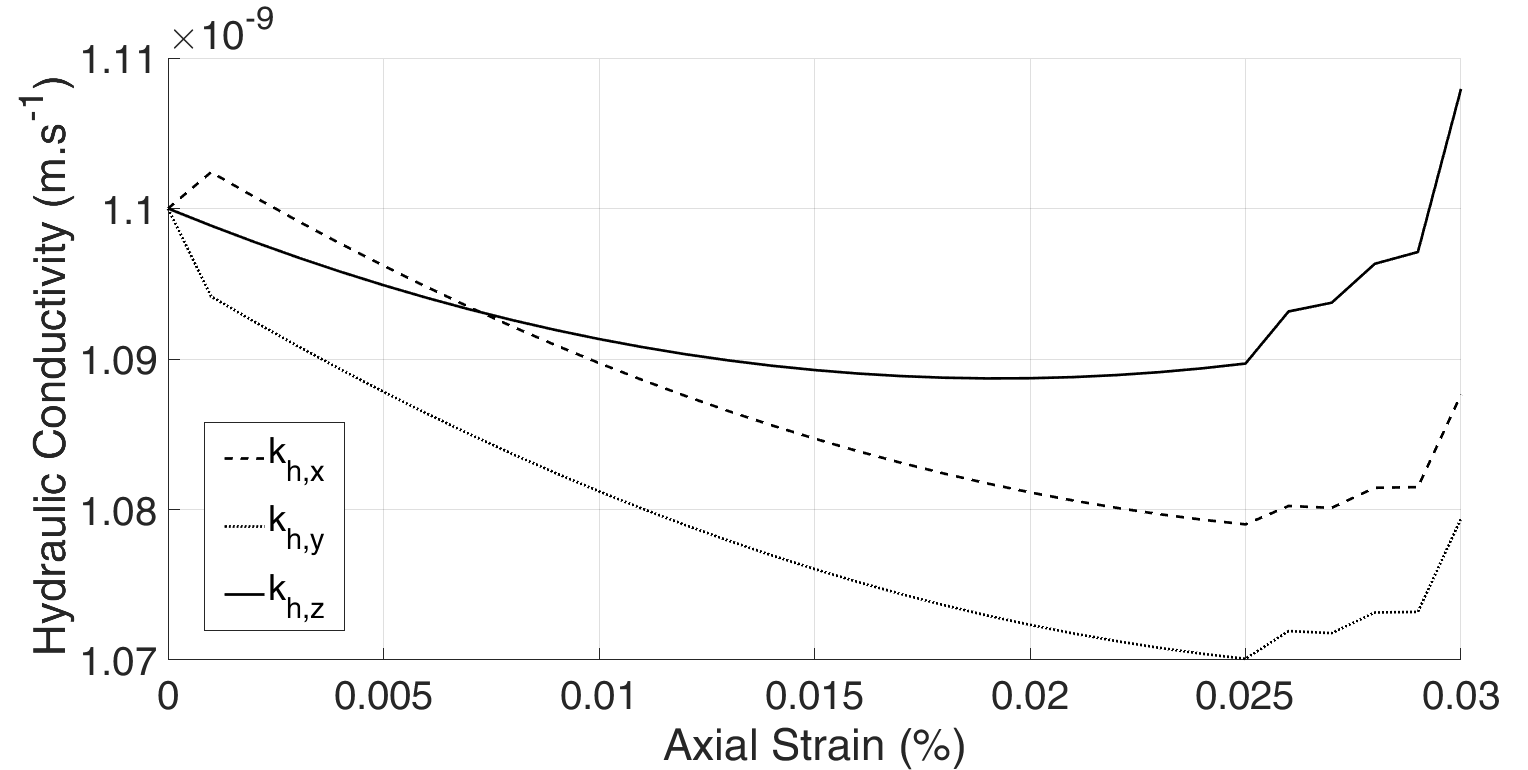
\includegraphics[width=0.85\textwidth]{figures/Amir_ME5_Lattice_Drying_Data.png}
\caption{The change of hydraulic conductivity with applied linear strains}
\label{fig:Amir_ME5_Lattice_Drying_Data}
\end{figure}

\clearpage
%---------------------------------------------------------
\subsubsection*{Meta Data Overview (according to Dublin Core)}
%---------------------------------------------------------

\begin{table}[!ht]
\caption{MEX 1-1 (CAU)}
\label{tab:dms-mex1-1b}
\small
\begin{tabular}{R{3.5cm}|L{7.5cm}}
\hline
%
Data label     & GeomInt - CAU - Swelling process, Red Salt Clay\\
URL (Numerics) &  \url{https://nextcloud.ifg.uni-kiel.de/index.php/s/JmZseQqrsbgWNqC} \\
Subject        &  Swelling process (Red Salt Clay)\\
Type of data   & Executable MATLAB P-file, input parameters\\
Data quality   &  Quality assured data \\
Status of data &  Unprocessed data\\
Data format    & txt, MATLAB executable P-file\\
Creators       &  Kiel University, Institute of Geomechanics and Geotechnics, Ludewig-Meyn-Stra\ss e 10, 24118, Kiel\\
Source/Origin  & In-house code \\
Publisher      & Kiel University, Institute of Geomechanics and Geotechnics, Ludewig-Meyn-Stra\ss e 10, 24118, Kiel \\
Rights holders & Kiel University, Institute of Geomechanics and Geotechnics, Ludewig-Meyn-Stra\ss e 10, 24118, Kiel \\
Contributors   & Kiel University, Institute of Geomechanics and Geotechnics: Amir Shoarian Sattari, Frank Wuttke\\
Time/period of creation & 2019-2020\\
Language of the content & English\\
Update policy           & Stored data is final\\
Access permissions      & Full access\\
%
\hline
\end{tabular}
\end{table}